% SPDX-FileCopyrightText: 2025 Jorge Teixeira Crespo <jorge.teixeira@udc.es>
%
% SPDX-License-Identifier: GPL-2.0-or-later

\chapter{Current Infrastructure Analysis}
\label{chap:current-infrastructure}

\lettrine{T}{his} chapter provides an in-depth analysis of GPUL's current server infrastructure, focusing on the two legacy servers: GPULINO and GPULON. These servers host critical services but also pose significant operational and maintenance challenges. GPULINO, created on November 3, 2011, and GPULON, launched on January 17, 2016, have remained largely unchanged since their deployment. The chapter reviews their specifications, configurations, and highlights key issues such as outdated software, inconsistent backup strategies, and the lack of proper documentation. It also discusses the impact of these limitations on GPUL's operations, underlining the urgent need for a comprehensive infrastructure renewal.

\section{GPULINO Server Analysis}

GPULINO is hosted with Gandi, located in their Paris, France (SD3 datacenter). It runs Debian GNU/Linux 8 (Jessie), which is significantly outdated as it reached End-of-Life (EOL) on June 17, 2018, with Extended LTS support ending on June 30, 2025.

\subsection{Technical Specifications}

GPULINO is a legacy virtual machine that remains in active use within the association's infrastructure. Provisioned in 2011, it has undergone minimal changes since its deployment. The table below summarizes its key specifications, which reflect the outdated and limited nature of the system. These constraints have direct implications for performance, maintenance, and security.

\begin{table}[H]
  \centering
  \rowcolors{2}{white}{udcgray!25}
  \caption{GPULINO Server Specifications}
  \label{tab:gpulino_specs}
  \begin{tabular}{ll}
    \rowcolor{udcpink!25}
    \textbf{Specification} & \textbf{Details} \\
    \hline
    CPU & 1 core \\
    RAM & 640 MB \\
    Storage & 3 x 10 GB volumes \\
    Monthly Cost & €13.09 \\
    IPv4 & 95.142.163.196 \\
    IPv6 & 2001:4b98:dc0:47:216:3eff:fe56:1785 \\
    OS & Debian GNU/Linux 8 (Jessie, EOL) \\
  \end{tabular}
\end{table}

\subsection{Filesystem Structure}

GPULINO uses three independent 10 GB volumes provided by the hosting provider. These are mounted as root (\verb|/|), data (\verb|/srv/srv_gpulino|), and backup (\verb|/srv/backup_gpulino|). Their current usage is visualized in Figure~\ref{fig:gpulino_disk_usage}.

\begin{figure}[H]
  \centering
  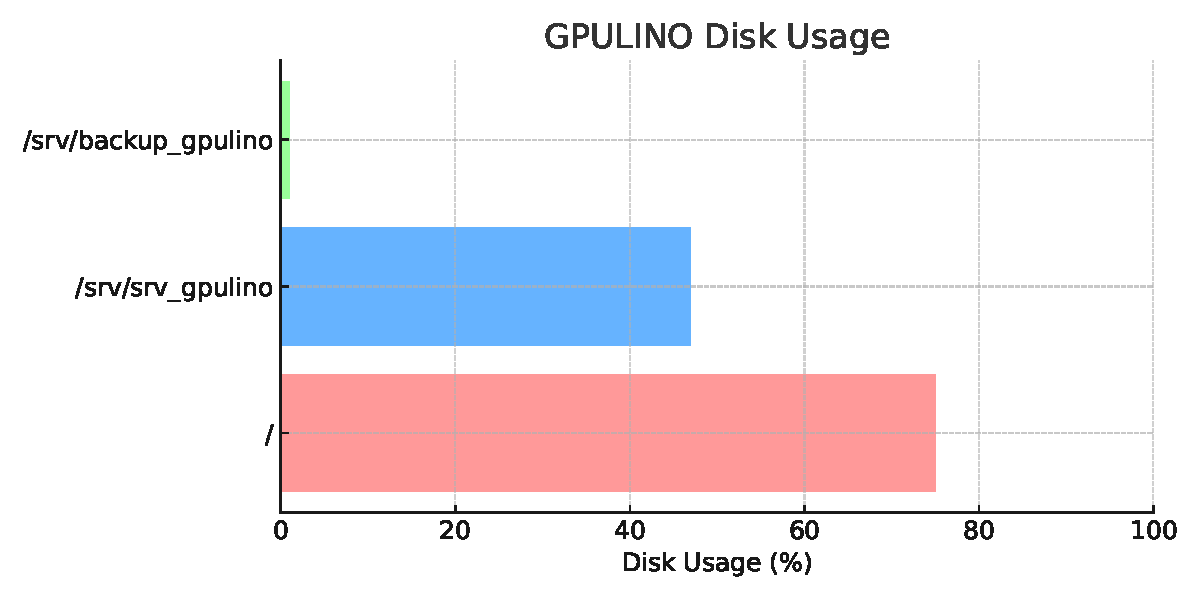
\includegraphics[width=0.7\textwidth]{figuras/gpulino_disk_usage.pdf}
  \caption{Disk usage across GPULINO volumes.}
  \label{fig:gpulino_disk_usage}
\end{figure}

While the root filesystem is nearing critical usage (~75\%), the backup volume remains largely underutilized (~1\%), showcasing the lack of backup strategy.

\subsection{User Access and Management}

The server maintains several user accounts, with varying levels of activity. Table \ref{tab:gpulino_users} shows the most relevant user logins:

\begin{table}[H]
  \centering
  \rowcolors{2}{white}{udcgray!25}
  \caption{GPULINO Active User Accounts (sorted by creation date)}
  \label{tab:gpulino_users}
  \begin{tabular}{ll}
    \rowcolor{udcpink!25}
    \textbf{Username} & \textbf{Last Login} \\
    \hline
    admin & September 26, 2020 \\
    tsao & September 27, 2024 \\
    ssaavedra & January 27, 2024 \\
    marcos.chavarria & February 19, 2014 \\
    castrinho8 & March 18, 2017 \\
    chema & April 24, 2019 \\
    teixe & January 19, 2025 \\
  \end{tabular}
\end{table}

\subsection{Active Services and Usage Details}

The server hosts several critical services:
\begin{itemize}
    \item Apache2 Web Server
    \item Exim4 Mail Transport Agent
    \item Mailman 2 (for mailing lists)
    \item MySQL (database server, supporting Mailman)
    \item SSH (Secure Shell)
\end{itemize}

Although these services were known to be active, GPULINO lacked formal documentation. A manual inspection of the server's filesystem and configuration files revealed various hosted domains, tools, and historical content.

The Apache configuration included several virtual hosts pointing to subdomains, some of which were no longer functional. Others still displayed static content or redirected to internal projects.

\begin{table}[H]
  \centering
  \rowcolors{2}{white}{udcgray!15}
  \caption{Web domains served by Apache on GPULINO}
  \label{tab:gpulino_apache_domains}
  \begin{tabular}{ll}
    \rowcolor{udcpink!25}
    \textbf{Domain} & \textbf{Notes} \\
    \hline
    \texttt{planet.gpul.org} & Hosts a blog or webpage \\
    \texttt{old.gpul.org} & Returns a PHP error \\
    \texttt{stuff.gpul.org} & Hosts a webpage \\
    \texttt{dudesconf.org} & Hosts a webpage (some links broken) \\
    \texttt{junoffice.gpul.org} & Returns an empty page \\
    Other domains & Serve the default Apache welcome page \\
  \end{tabular}
\end{table}

These domains pointed to directories inside \texttt{/var/www}, which contained a variety of static and symlinked content likely tied to past events, services, or internal documentation.

\begin{table}[H]
  \centering
  \rowcolors{2}{white}{udcgray!15}
  \caption{Apache web directories found under \texttt{/var/www}}
  \label{tab:gpulino_www_dirs}
  \begin{tabular}{ll}
    \rowcolor{udcpink!25}
    \textbf{Directory} & \textbf{Description} \\
    \hline
    apache-default & Default Apache content \\
    artwork & Publicly accessible artwork files \\
    drupal & Linked to \texttt{/var/www/gpul.org/drupal} \\
    dudesconf & Hosts content for dudesconf.org \\
    estatutos & Organizational rules or statutes \\
    etherpad-lite & Likely collaborative editor \\
    eventostuff & Linked to \verb|/srv/srv_gpulino/eventos| \\
    gallery2 & Public gallery \\
    gpul-latex & LaTeX-related files \\
    gpul.org & Main content for GPUL \\
    gpul.org-eventos & Event-specific content \\
    guademy & Linked to \verb|/srv/srv_gpulino/www/guademy/| \\
    indico & Linked to \verb|/srv/srv_gpulino/indico| \\
    junoffice & Content for junoffice.gpul.org \\
    labs.gpul.org & Lab-related subdomain \\
    piwik & Web analytics platform \\
    planet.gpul.org & Static site content \\
    rexistro.labs.gpul.org & Registry or logs \\
    votologo & Likely a voting tool \\
  \end{tabular}
\end{table}

Mailman was configured to manage mailing lists under the \texttt{lists.gpul.org} domain, using a CGI interface and Apache redirection rules. The configuration was minimal but functional.

\begin{table}[H]
  \centering
  \rowcolors{2}{white}{udcgray!15}
  \caption{Mailman service details on GPULINO}
  \label{tab:gpulino_mailman}
  \begin{tabular}{ll}
    \rowcolor{udcpink!25}
    \textbf{Parameter} & \textbf{Value} \\
    \hline
    Domain & \texttt{lists.gpul.org} \\
    VirtualHost & Redirects root to \texttt{/cgi-bin/mailman/listinfo} \\
    CGI Path & \texttt{/usr/lib/cgi-bin/} \\
    DocumentRoot & \texttt{/var/www/} \\
    Admin Email & \texttt{mailman@lists.gpul.org} \\
  \end{tabular}
\end{table}

The server also ran a Git daemon that served multiple repositories under a single base path. These were accessible via the \texttt{git://} protocol and configured to run from a root-owned script.

\begin{table}[H]
  \centering
  \rowcolors{2}{white}{udcgray!15}
  \caption{Git daemon configuration details}
  \label{tab:gpulino_git_daemon}
  \begin{tabular}{ll}
    \rowcolor{udcpink!25}
    \textbf{Parameter} & \textbf{Value} \\
    \hline
    Startup Script & \texttt{/root/git-daemon} \\
    Base Path & \verb|/srv/srv_gpulino/git/repositories/| \\
  \end{tabular}
\end{table}

\noindent
\textbf{Git Daemon Command:}

\begin{lstlisting}[language=sh]
/usr/bin/git-daemon \
  --user=git --group=git \
  --verbose \
  --reuseaddr \
  --base-path=/srv/srv_gpulino/git/repositories/ \
  /srv/srv_gpulino/git/repositories/
\end{lstlisting}

\begin{table}[H]
  \centering
  \rowcolors{2}{white}{udcgray!15}
  \caption{Git repositories hosted}
  \label{tab:gpulino_git_repos}
  \begin{tabular}{ll}
    \rowcolor{udcpink!25}
    \textbf{Repository} & \textbf{Description} \\
    \hline
    \texttt{actas.git} & Meeting minutes \\
    \texttt{certificado-asistencia.git} & Attendance certificates \\
    \texttt{cuentas.git} & Financial records \\
    \texttt{gitosis-admin.git} & Git access management \\
    \texttt{gpul-estatutos.git} & Organization statutes \\
    \texttt{manual-latex.git} & LaTeX training material \\
    \texttt{mem-dudesconf.git} & DudesConf report \\
    \texttt{parte-gasto.git} & Expense reports \\
    \texttt{subvencion-udc-2011.git} & UDC grant files (2011) \\
  \end{tabular}
\end{table}

These findings illustrate the range of active uses the server had, many of which were not documented but still functional at the time of analysis. They also reflect the historical depth and variety of GPUL's activities over the years.

\section{GPULON Server Analysis}

GPULON is hosted with Kimsufi and configured as a KS-4C server running Debian GNU/Linux 11 (Bullseye).

\subsection{Technical Specifications}

\begin{table}[H]
  \centering
  \rowcolors{2}{white}{udcgray!25}
  \caption{GPULON Server Specifications}
  \label{tab:gpulon_specs}
  \begin{tabular}{ll}
    \rowcolor{udcpink!25}
    \textbf{Specification} & \textbf{Details} \\
    \hline
    CPU & Intel i5-2300 \\
    RAM & 16 GB \\
    Storage & 1 x 2TB HDD \\
    Monthly Cost & €30.60 \\
    IPv4 & 91.121.65.91 \\
    OS & Debian GNU/Linux 11 (Bullseye) \\
  \end{tabular}
\end{table}

\subsection{Filesystem Structure}

GPULON has a single 2 TB physical disk, divided into logical volumes for \texttt{/home}, \texttt{/var/lib/docker}, and the root filesystem (\texttt{/}). This setup is visualized in Figure~\ref{fig:gpulon_disk_usage}.

\begin{figure}[H]
  \centering
  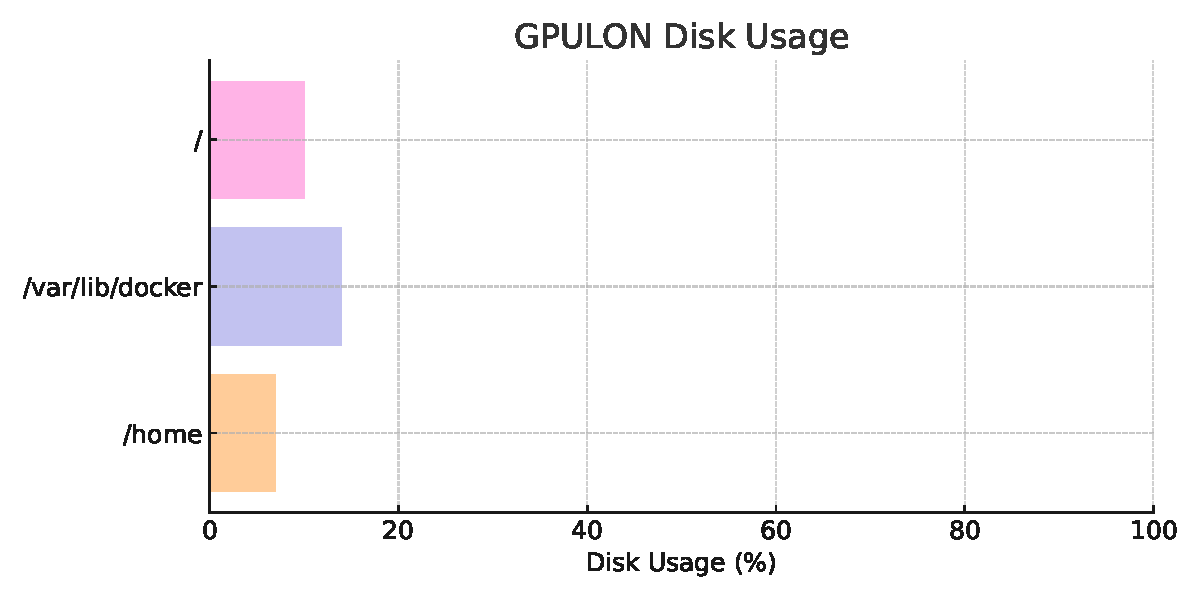
\includegraphics[width=0.7\textwidth]{figuras/gpulon_disk_usage.pdf}
  \caption{Disk usage across GPULON logical volumes after reallocation.}
  \label{fig:gpulon_disk_usage}
\end{figure}

Originally, the Docker directory (\texttt{/var/lib/docker}) had been restricted to approximately 450 GB and became rapidly saturated, primarily due to logs generated by long-running containerized services. One Nextcloud log file alone exceeded 250 GB.

This issue caused an operational incident that affected system stability. Resolving it involved manually deleting the oversized log and reallocating disk space to expand the Docker volume.

The updated logical volume allocation now stands as follows:

\begin{itemize}
    \item \texttt{/home} — 272 GB (7\% usage)
    \item \texttt{/var/lib/docker} — 1.5 TB (14\% usage)
    \item Root filesystem (\texttt{/}) — 58 GB (10\% usage)
\end{itemize}

This reallocation has significantly improved headroom for service logs and application data, reducing the risk of similar incidents in the future.

\subsection{User Access and Management}

Table \ref{tab:gpulon_users} shows the active user accounts on GPULON:

\begin{table}[H]
  \centering
  \rowcolors{2}{white}{udcgray!25}
  \caption{GPULON Active User Accounts (sorted by creation date)}
  \label{tab:gpulon_users}
  \begin{tabular}{ll}
    \rowcolor{udcpink!25}
    \textbf{Username} & \textbf{Last Login} \\
    \hline
    root & January 17, 2016 \\
    ssaavedra & April 1, 2025 \\
    castrinho8 & September 25, 2020 \\
    davidmaseda & August 22, 2023 \\
    bruno.cabado & August 9, 2024 \\
    tsao & October 1, 2023 \\
    pedro.costal & March 27, 2022 \\
    teixe & May 17, 2025 \\
    delthia & March 29, 2025 \\
  \end{tabular}
\end{table}

\subsection{Docker Environment}

GPULON primarily uses Docker for service deployment, hosting:
\begin{itemize}
  \item Nextcloud (cloud suite platform)
  \item Listmonk (email marketing platform)
  \item Activepieces (automation platform)
  \item Traefik (reverse proxy)
  \item Various supporting databases (Postgres, Redis, MariaDB)
\end{itemize}

\section{Critical Issues and Challenges}

Although GPUL's servers are still running, they have many problems that make them hard to maintain and unreliable. Over time, different people have made changes without clear planning or documentation, which has led to a fragile system. This section describes the main problems we found, divided into two groups: serious issues that affect how the servers work, and general problems with how the infrastructure is set up.

\subsection{Known Critical Issues}

The current infrastructure presents several critical issues:
\begin{itemize}
  \item \textbf{OS Obsolescence}: GPULINO is severely outdated, running an EOL operating system.
  \item \textbf{Nextcloud Obsolescence}: The Nextcloud version used is 24.0.6, which is no longer maintained. The latest is version 32.
  \item \textbf{Manual Interventions}: Critical services require manual restart post-reboot.
  \item \textbf{Insufficient Backup Strategy}: No systematic backup; sporadic manual backups to personal NAS.
  \item \textbf{Lack of Automated Log Rotation}: Manual log maintenance required, causing periodic instability.
\end{itemize}

\subsection{Known Infrastructure Issues}

Additional challenges include:
\begin{itemize}
  \item \textbf{Docker Misconfiguration (GPULON)}: The \texttt{/srv/docker} directory has grown into a chaotic collection of loosely organized folders and services, with multiple Docker Compose files scattered across subdirectories in inconsistent ways. There is little to no documentation, naming is irregular, and services are grouped without a clear structure, making it extremely difficult to understand what is running or how components are connected.
  \item \textbf{Unknown Installed Services (GPULINO)}: Legacy services were poorly documented, making it difficult to determine what was hosted or how services were configured. Understanding the system required inspection of configuration files, web directories, and service logs, effectively a detailed forensic review akin to a forensic investigation.
\end{itemize}

\section{Impact on Operations}


GPUL's current infrastructure has already caused serious disruptions to the organization's daily operations. These issues are not only technical, they affect how GPUL communicates, plans events, and meets important deadlines. A clear example of this is the ongoing trouble with the email system. GPUL uses redirects for several critical email addresses under the \texttt{gpul.org} domain. However, this setup often causes messages to be marked as spam. As a result, important emails related to event organization, sponsors, or participants are sometimes not delivered or go unnoticed, making coordination much harder.

Another major incident occurred when the GPULON server became unresponsive due to unrotated log files completely filling up the server's disk. This failure happened just before the end of a financial quarter, a key moment for administrative tasks. Resolving the issue took four days, required assistance from the external hosting provider, and placed GPUL at risk of missing key reporting deadlines. This event highlighted the fragility and poor maintainability of the current system, and how technical problems can quickly become organizational ones.
